% -*- TeX-master: "User_guide"; fill-column: 75 -*-

\chapter{JSBML Extensions Overview}
\label{sec:extensionsOverview}

In this chapter, we quickly overview the \SBMLthree packages currently
implemented for JSBML.

\section{Qualitative Models Package}
\label{sec:qual-overview}

Qualitative Models package (qual, for short) allows species in a model to 
have non-quantitative or non-continuous concentrations (Chaouiya et al., 2013). 
This may manifest as Boolean or discrete values, and is primarily employed in 
modeling gene regulation, sig-naling pathways, and metabolic networks using 
logical/Boolean networks (Schmulevich et al., 2002) or Petri nets 
(Breitling et al., 2008), which in turn, do not rely on traditional quantitative
coeffi-cients to encode relationships between biochemical entities.

\begin{figure}[hb]
 \centering
 \vspace*{2ex}
 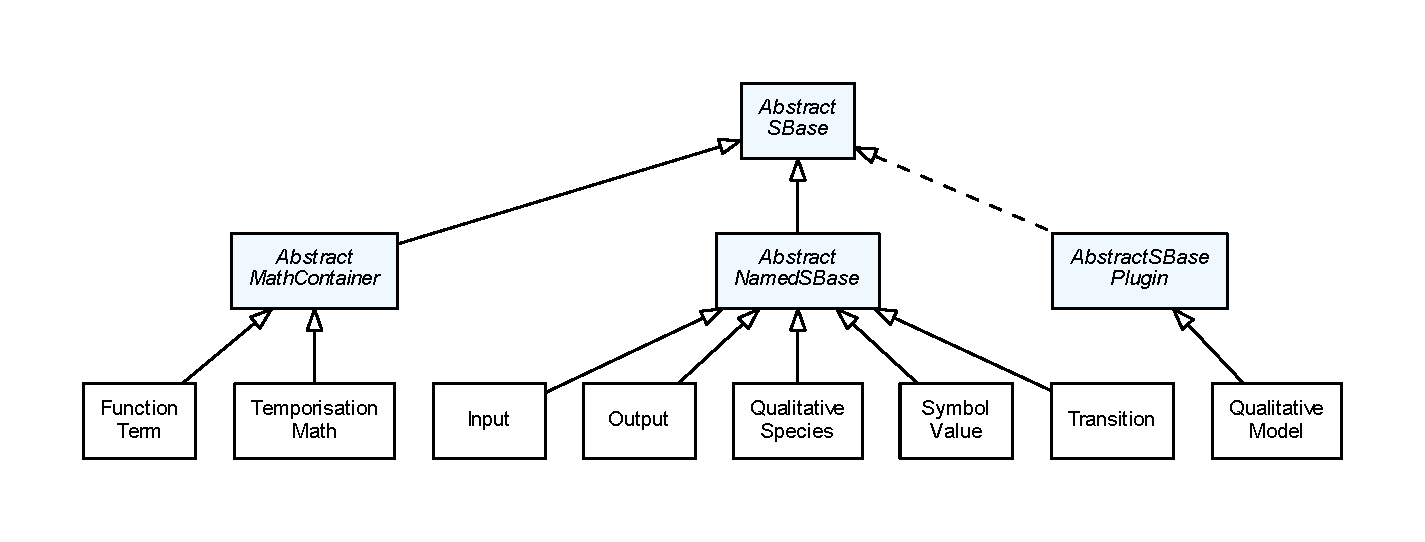
\includegraphics[width=\textwidth]{../../../extensions/qual/doc/img/type_hierarchy.pdf}
 \caption[The qualitative models extension]{}
 \label{fig:qual}
\end{figure}

\section{Flux Balance Constraints Package}
\label{sec:fbc-overview}
Constraints based modeling (Lewis et al., 2012) utilizes a class of models in which
the canonical stoichiometric relations between reac-tions and metabolites are specified
as constraints for convex analysis and mathematical optimization. Although species,
reactions, and stoichiometry can be encoded using the SBML L3V1,
Flux Balance Constraints (fbc, Olivier and Bergmann, 2013) enable a constraints
based perspective. For example, the constraints based approach called
Flux Balance Analysis (FBA) often aims to find the maximum growth rate of the
cell given a set of uptake possibilities and the ratio of molecules needed
for cell growth. The mathematical formulation for this optimization problem
has variables of reaction fluxes and constraints of mass balances around the
metabolites and bounds on the variable reaction fluxes. Because this formulation is
underdetermined, an objective, usually one that maximizes a biomass function which
corresponds to growth rate, is supplied which optimizes the reaction fluxes. Therefore,
the fbc package extends the SBML Level 3 core to specifically encode for bounds on
fluxes, constraints, and objective functions, which facilitates a fluid interface to
existing constraints based modeling software and optimization solvers.

\begin{figure}[hb]
 \centering
 \vspace*{2ex}
 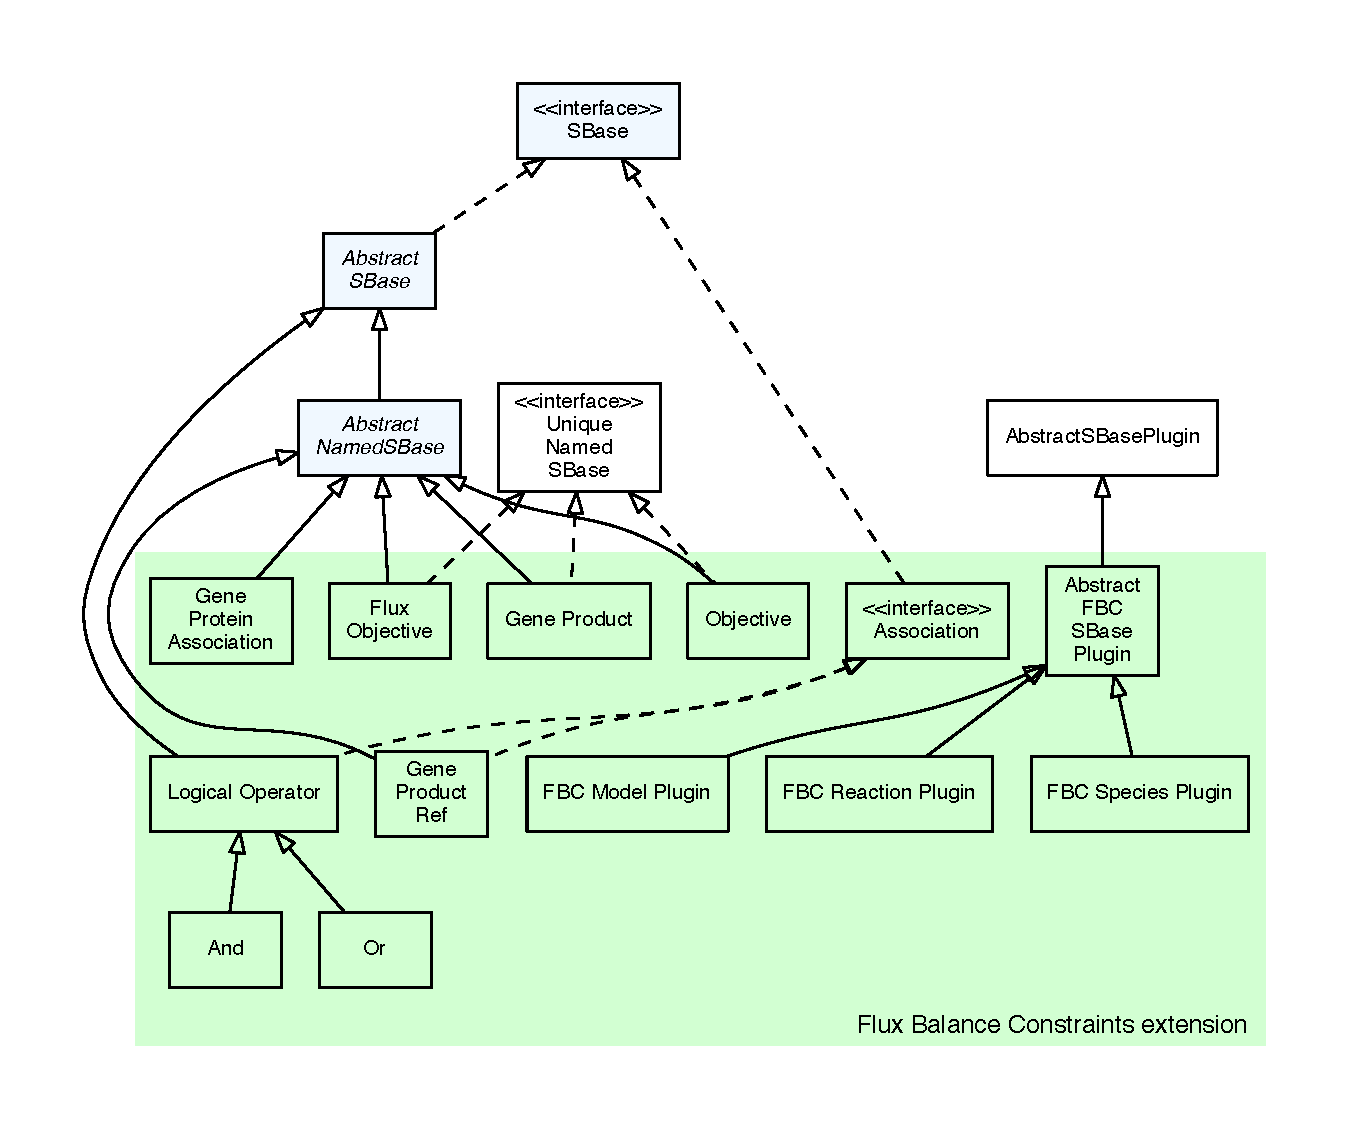
\includegraphics[width=\textwidth]{../../../extensions/fbc/doc/img/type_hierarchy.pdf}
 \caption[The flux balance constraints extension]{}
 \label{fig:fbc}
\end{figure}

\section{Layout Package}
\label{sec:layout-overview}

SBML encodes a core set of components (species, reactions) that make up
biochemical networks. The layout extension supports specifying graphical
information for these components. The structure for this extension mirrors 
the SBML Level 3 core hierarchy by introducing graphical object (glyph)
counterparts to reactions and species. Glyphs can optionally correspond
to elements in standard SBML, and there can be many glyphs for one element.
In addition, layout elements of non-standard model components can be specified
using the generic GraphicalObject class. Although this exten-sion is powerful
enough to encode the position of all biochemically related graph components,
it should be noted that the scope of this package does not include rendering
of these components. This functionality is provided by the Render package.
Ultimately, the layout extension provides a common language that biochemical
graph editors and viewers can utilize to couple a model to a graph layout.

\begin{figure}[hb]
 \centering
 \vspace*{2ex}
 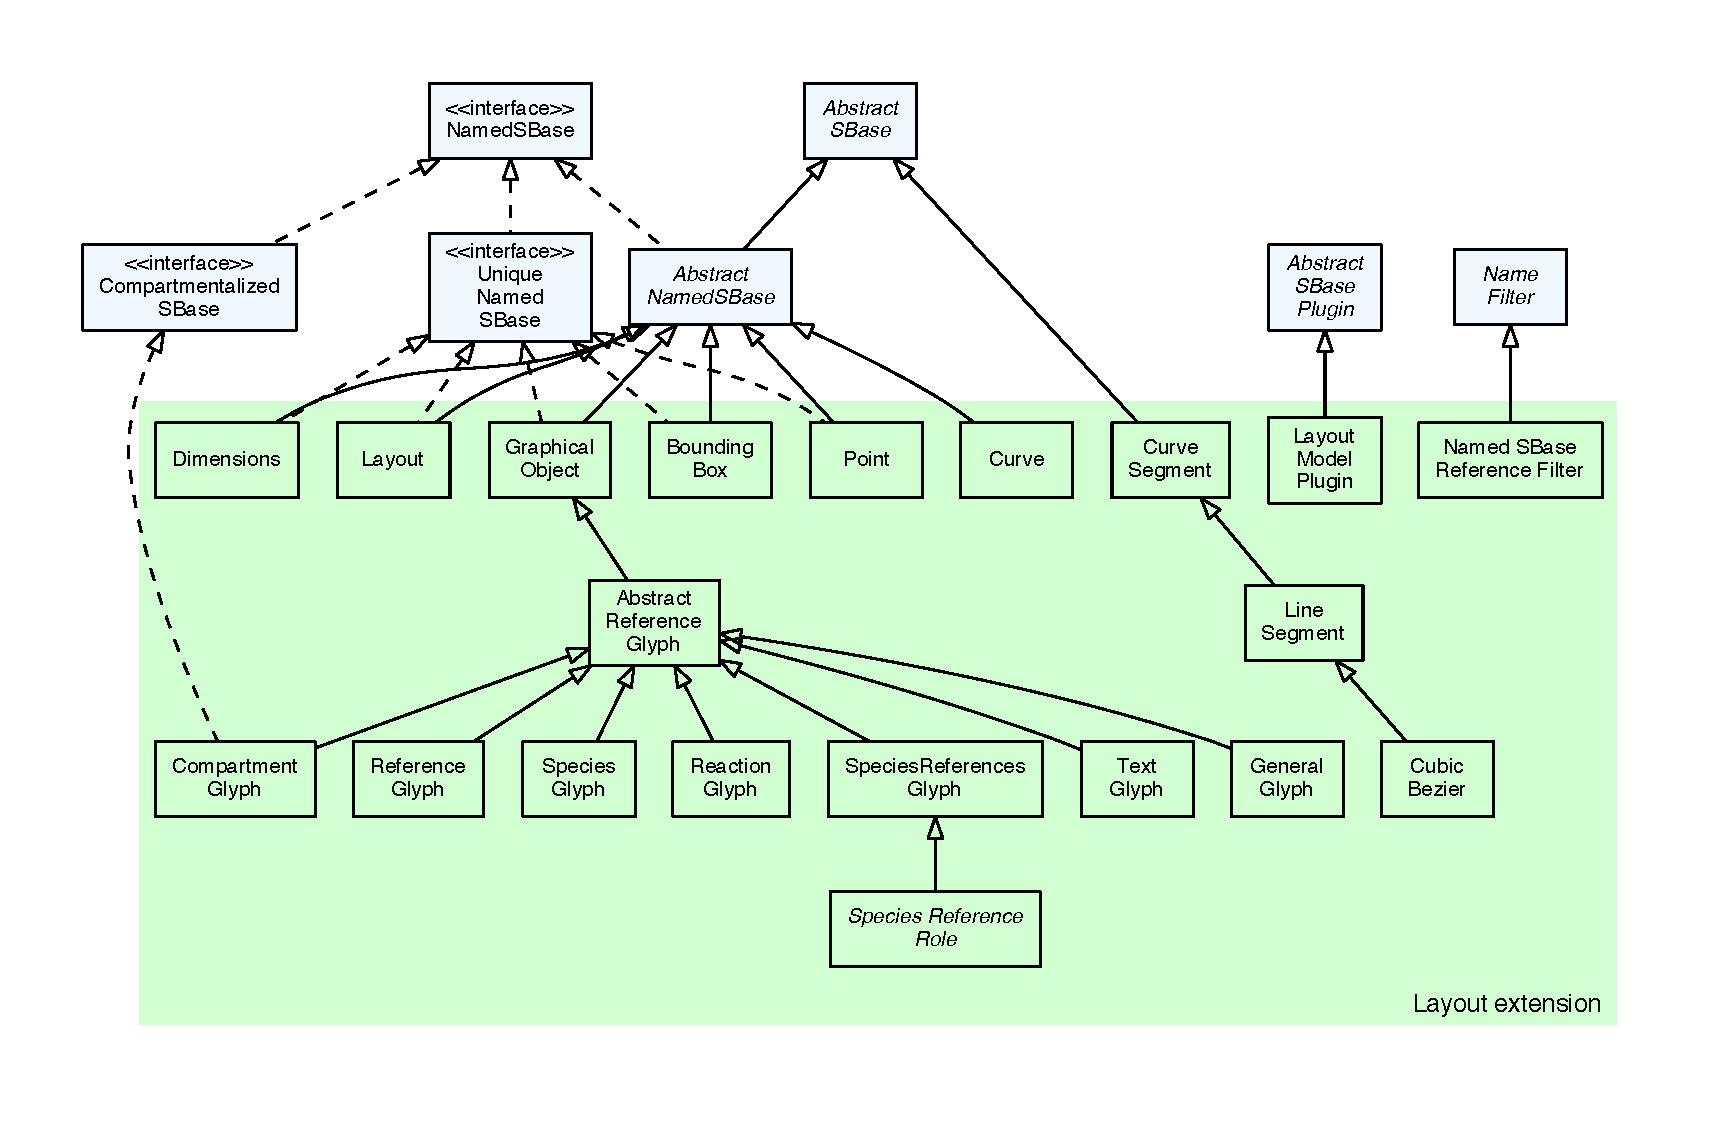
\includegraphics[width=\textwidth]{../../../extensions/layout/doc/img/type_hierarchy.pdf}
 \caption[The layout extension]{}
 \label{fig:layout}
\end{figure}

\section{Hierarchical Model Composition Package}
\label{sec:comp-overview}
As the amount of information for biochemical networks increases, models tend to
increase in complexity as well. The Hierarchical Model Composition extension (comp; Smith et al., 2013)
attempts to contextualize this complexity by providing a generic framework to encode
models as hierarchical entities in an SBML document. This functionality also allows
for storing multiple instances of a model within an enclosing model or document, which
can be used to build libraries of models within a document or to independently manage
different parts of a large model. Classes allow modelers to access elements within
sub-models and interface with other submodels, and comp provides a standardized approach
to define submodel differences with respect to parent or reference models. Overall, comp
is a powerful exten-sion to the SBML Level 3 core that gives modelers and programmers
options to standardize the encoding of complex, modular modeling frameworks. 

\begin{figure}[hb]
 \centering
 \vspace*{2ex}
 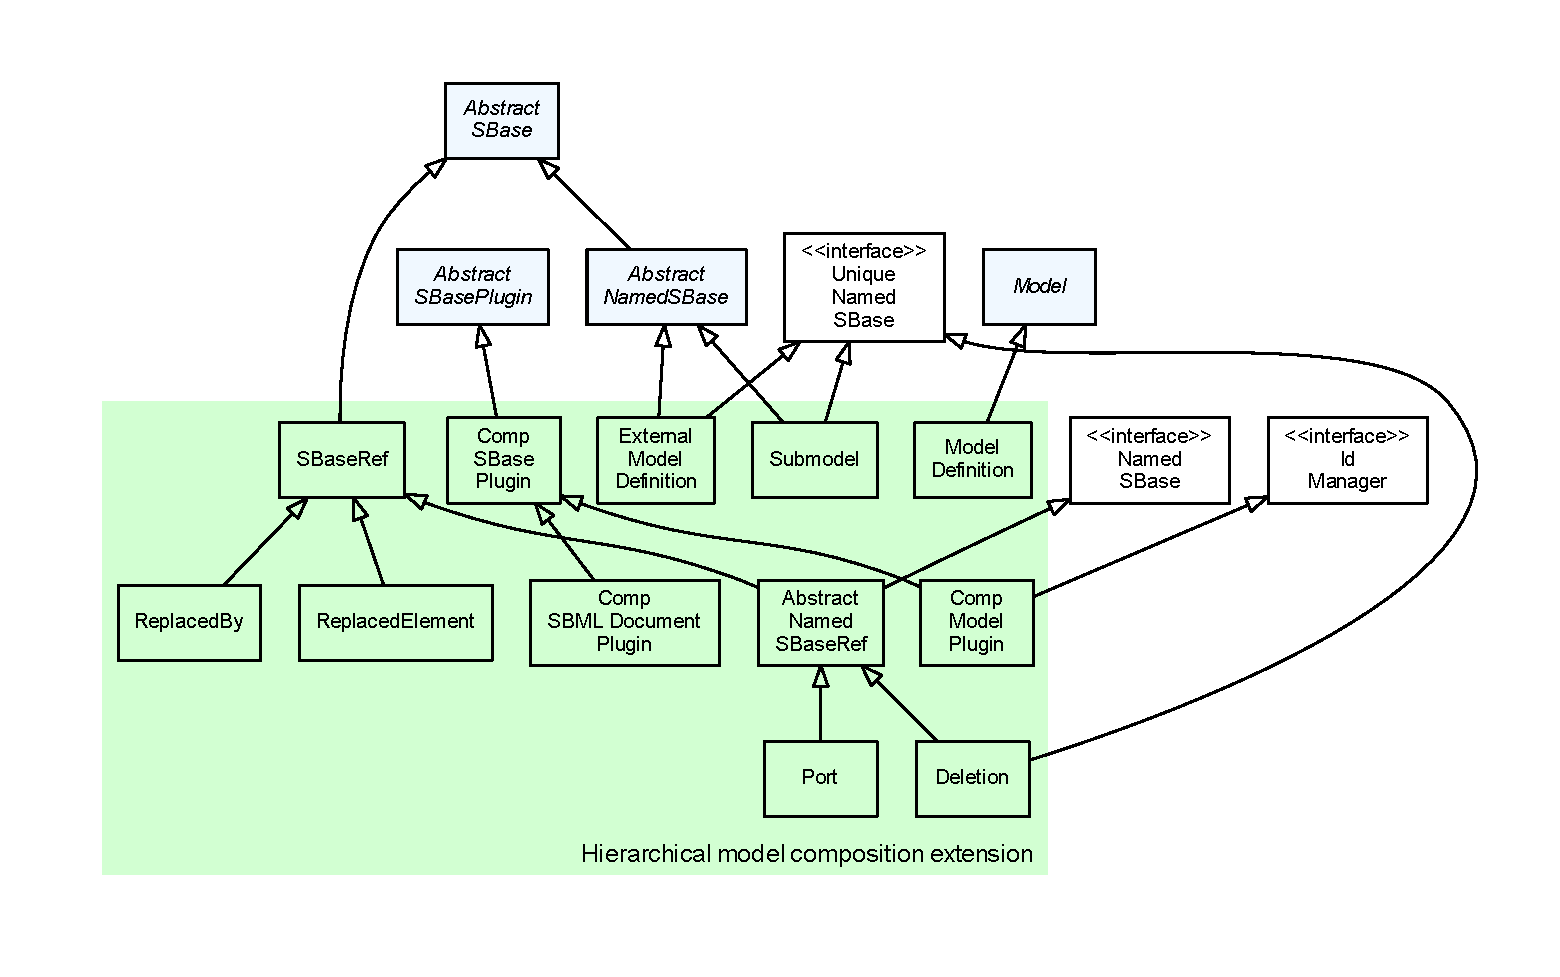
\includegraphics[width=\textwidth]{../../../extensions/comp/doc/img/type_hierarchy.pdf}
 \caption[The hierarchical model composition extension]{}
 \label{fig:comp}
\end{figure}

\section{Spatial Processes Package}
\label{sec:comp-overview}
The Spatial Processes extension (spatial, Schaff et al., 2014)
provides the ability to the SBML Level 3 core to specify subcellular,
geometric locations for components in biochemical
models. Although subcellular locations can be abstractly represented via
compartments in the SBML core specifica-tions, spatial enables the encoding of
a cellular coordinate system which can describe non-uniform molecular distributions,
diffusive transport, and spatially localized reactions. The Geometry class holds
the spatial information and the extended Species, Reaction, Compartment, and
Parameter objects have mappings to the spatial objects that hold information on
molecular transport coefficients, geometric domains, and coordinates. Spatial is
therefore able to store the geometric information commonly used in spatial modeling
tools for the biochemical entities from standard SBML.

\begin{figure}[hb]
 \centering
 \vspace*{2ex}
 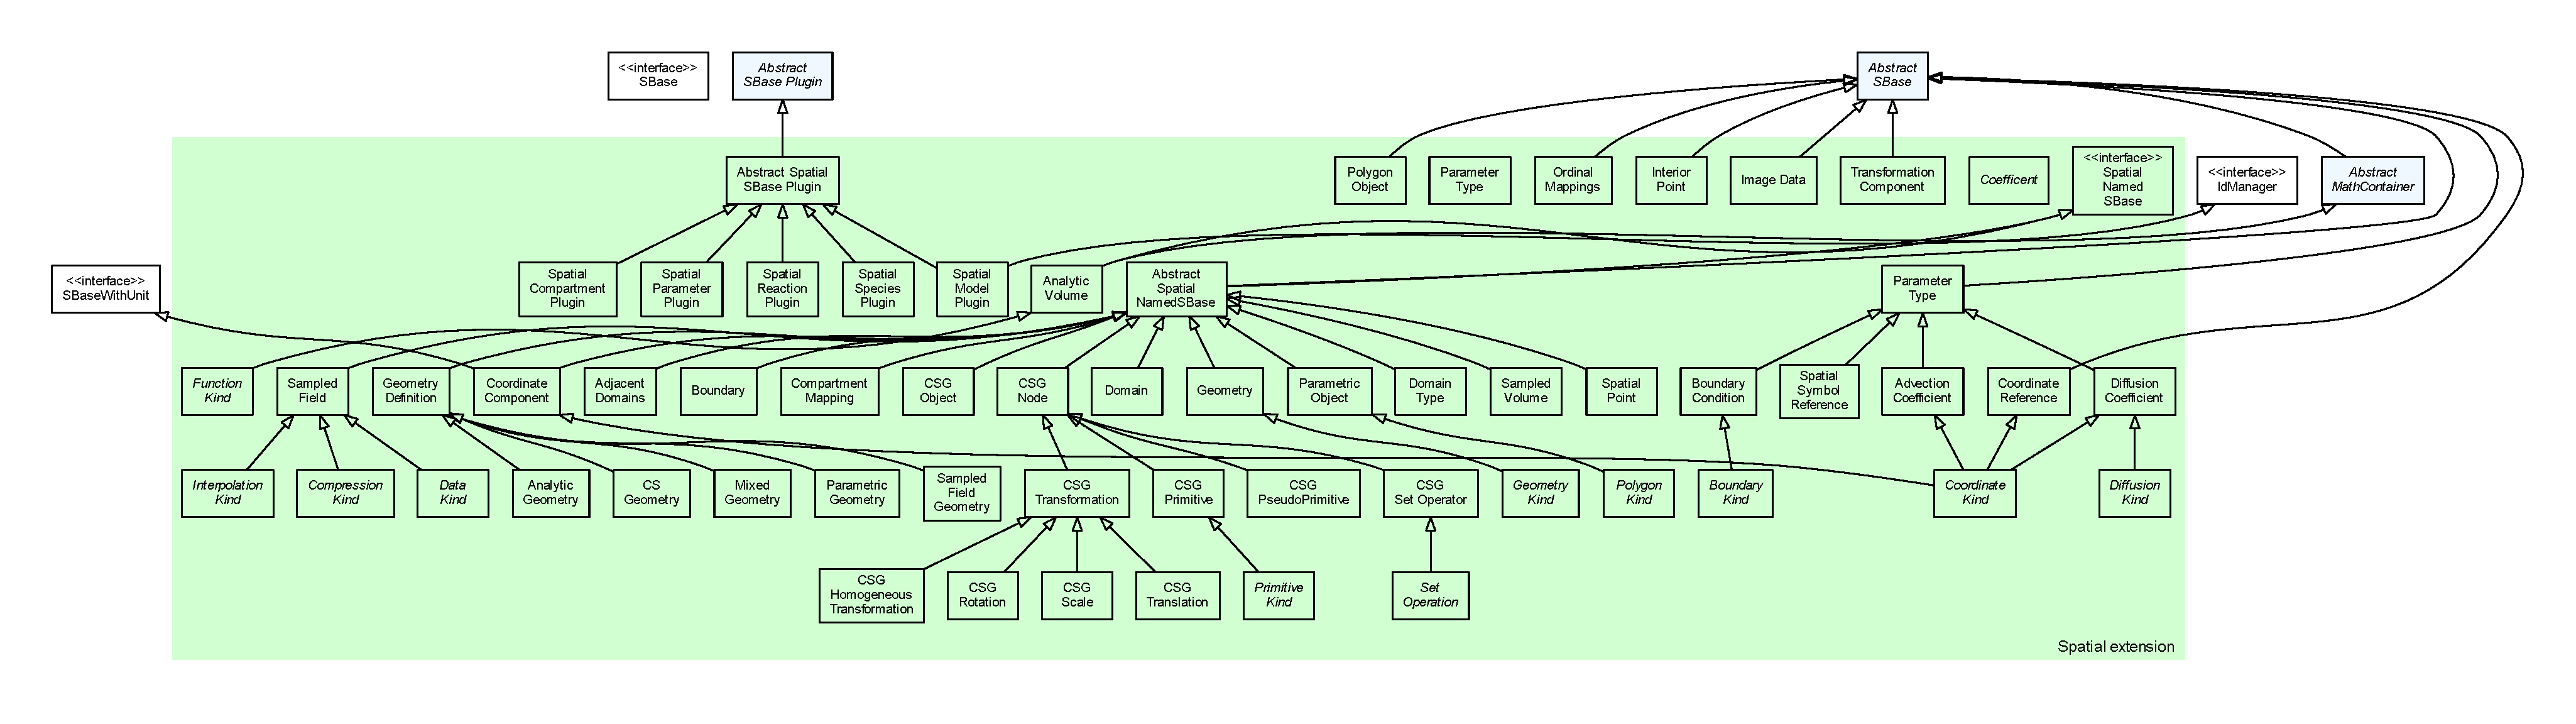
\includegraphics[width=\textwidth]{../../../extensions/spatial/doc/img/type_hierarchy.pdf}
 \caption[The spatial processes extension]{}
 \label{fig:spatial}
\end{figure}


\section{Groups Package}
\label{sec:groups-overview}
The other draft extension that is fully supported by JSBML is groups. 
This a small extension links together elements in an SBML model. Coupling
groups information with annotation and SBO terms (Courtot et al., 2011) 
contextualizes these sets of objects for properly conveying roles of groups 
for other programmers and modelers.

\begin{figure}[hb]
 \centering
 \vspace*{2ex}
 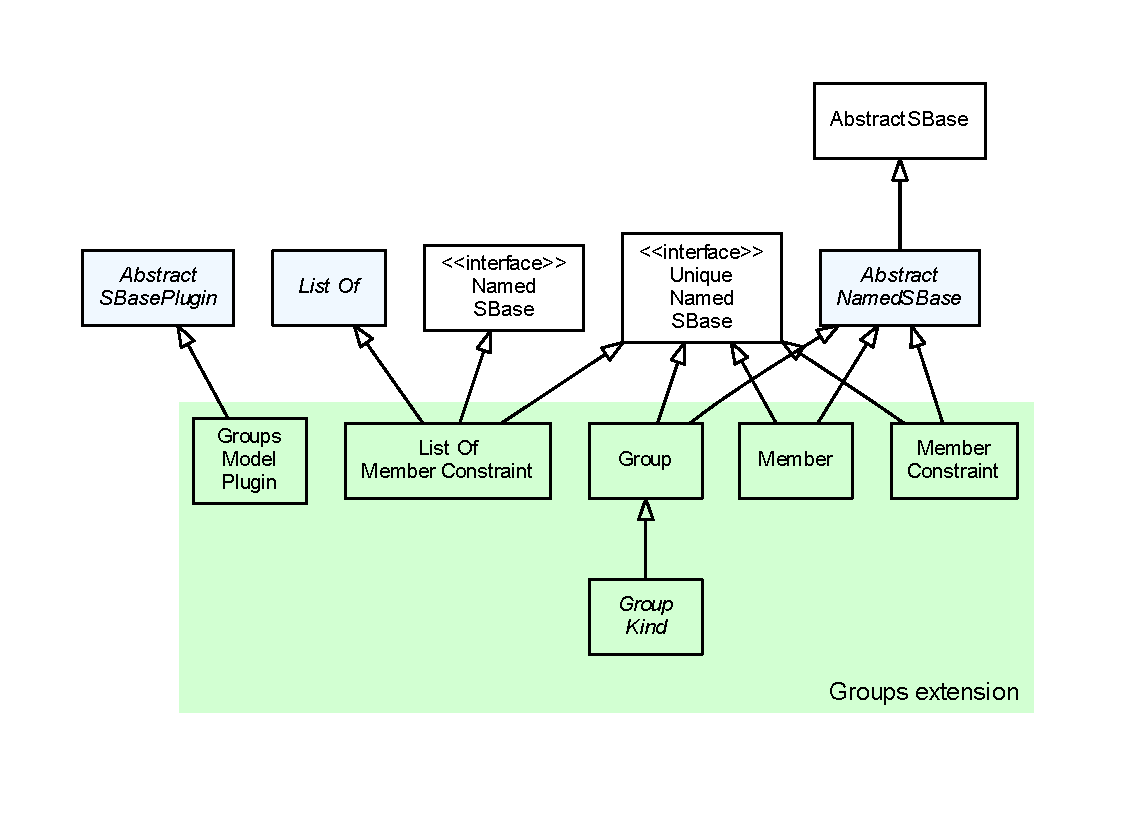
\includegraphics[width=\textwidth]{../../../extensions/groups/doc/img/type_hierarchy.pdf}
 \caption[The groups extension]{}
 \label{fig:groups}
\end{figure}


\section{Arrays Package}
\label{sec:arrays-overview}
Arrays (arrays, Watanabe et al., 2013) extends SBML variables to include arrays of values,
thereby representing repeated or regular model structures more efficiently.
Arrays provides the ability to access sets of values with indices instead of explicit
declaration and creation of sub-data objects.

\begin{figure}[hb]
 \centering
 \vspace*{2ex}
 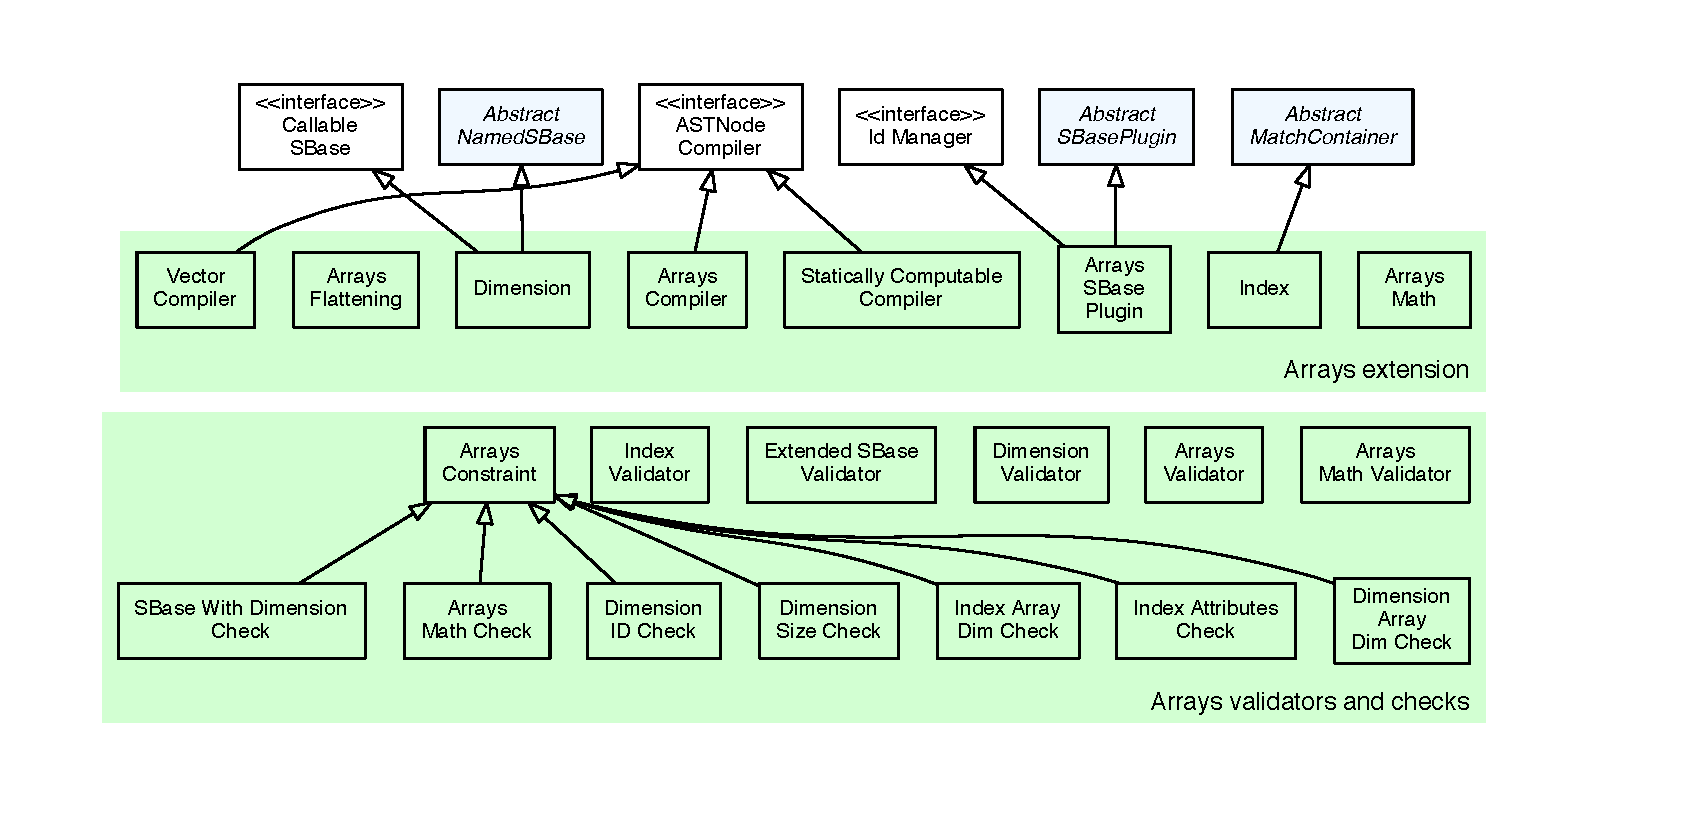
\includegraphics[width=\textwidth]{../../../extensions/arrays/doc/img/type_hierarchy.pdf}
 \caption[The arrays extension]{}
 \label{fig:arrays}
\end{figure}

\section{Required Elements Package}
\label{sec:req-overview}
Required Elements (req, Smith and Hucka, 2013) allows a model to indicate which
components have had their mathematical meanings changed by (e.g.) the use of
another SBML package.

\begin{figure}[hb]
 \centering
 \vspace*{2ex}
 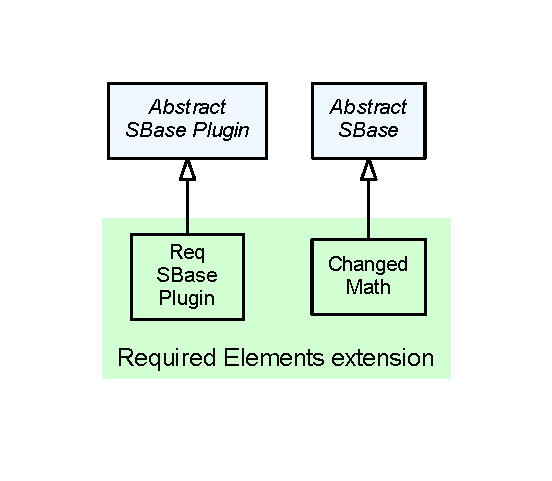
\includegraphics[width=\textwidth]{../../../extensions/req/doc/img/type_hierarchy.pdf}
 \caption[The arrays extension]{}
 \label{fig:arrays}
\end{figure}


\section{Distributions Package}
\label{sec:distrib-overview}
Distributions (distrib, Moodie and Smith, 2013) encodes
statistical distributions and their sampling.

\begin{figure}[hb]
 \centering
 \vspace*{2ex}
 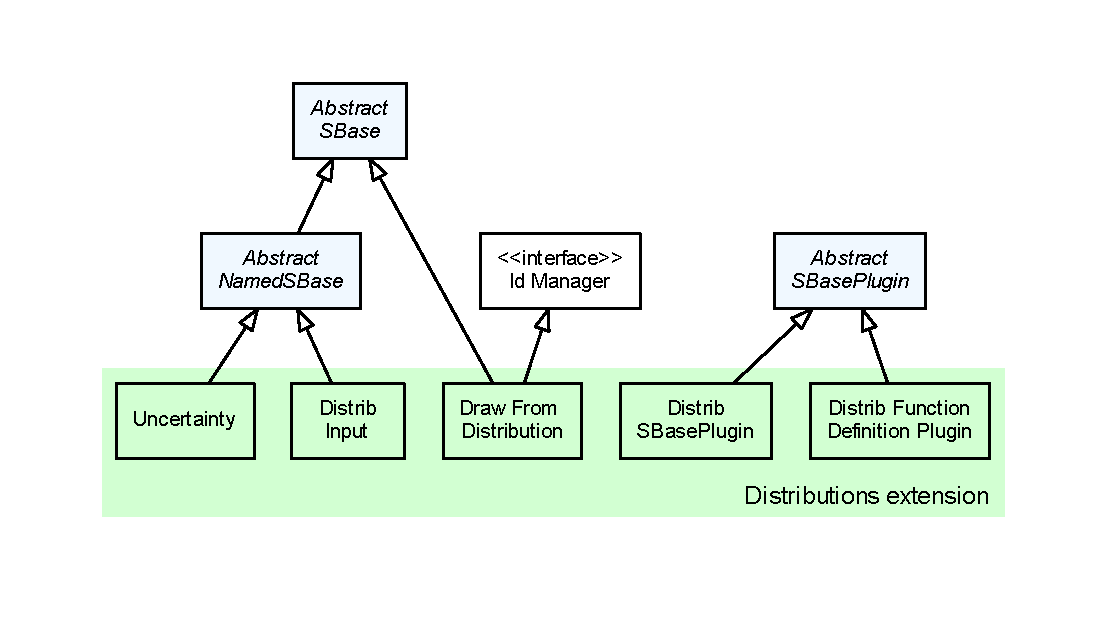
\includegraphics[width=\textwidth]{../../../extensions/distrib/doc/img/type_hierarchy.pdf}
 \caption[The distributions extension]{}
 \label{fig:distrib}
\end{figure}


\section{Dynamic Structures Package}
\label{sec:dyn-overview}
Dynamic Structures (dyn, Gomez et al., 2014), supports the definition
of dynamical behaviors for model entities.

\begin{figure}[hb]
 \centering
 \vspace*{2ex}
 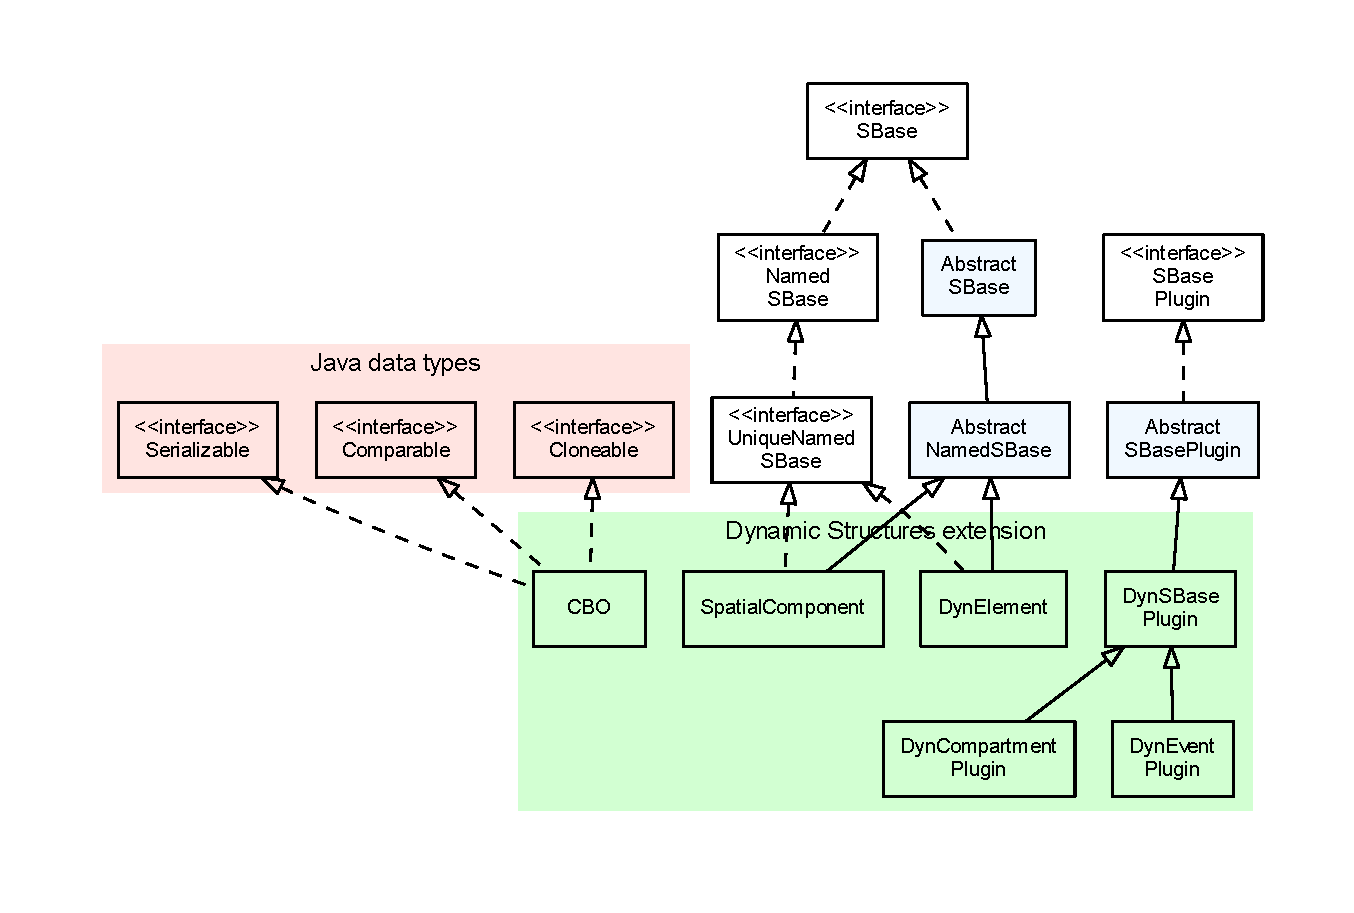
\includegraphics[width=\textwidth]{../../../extensions/dyn/doc/img/type_hierarchy.pdf}
 \caption[The dynamic structures extension]{}
 \label{fig:dyn}
\end{figure}


\section{Rendering Package}
\label{sec:render-overview}
Rendering (render, Gauges et al., 2011) couples with Layout to provide 
symbol and style information for network diagrams.

\begin{figure}[hb]
 \centering
 \vspace*{2ex}
 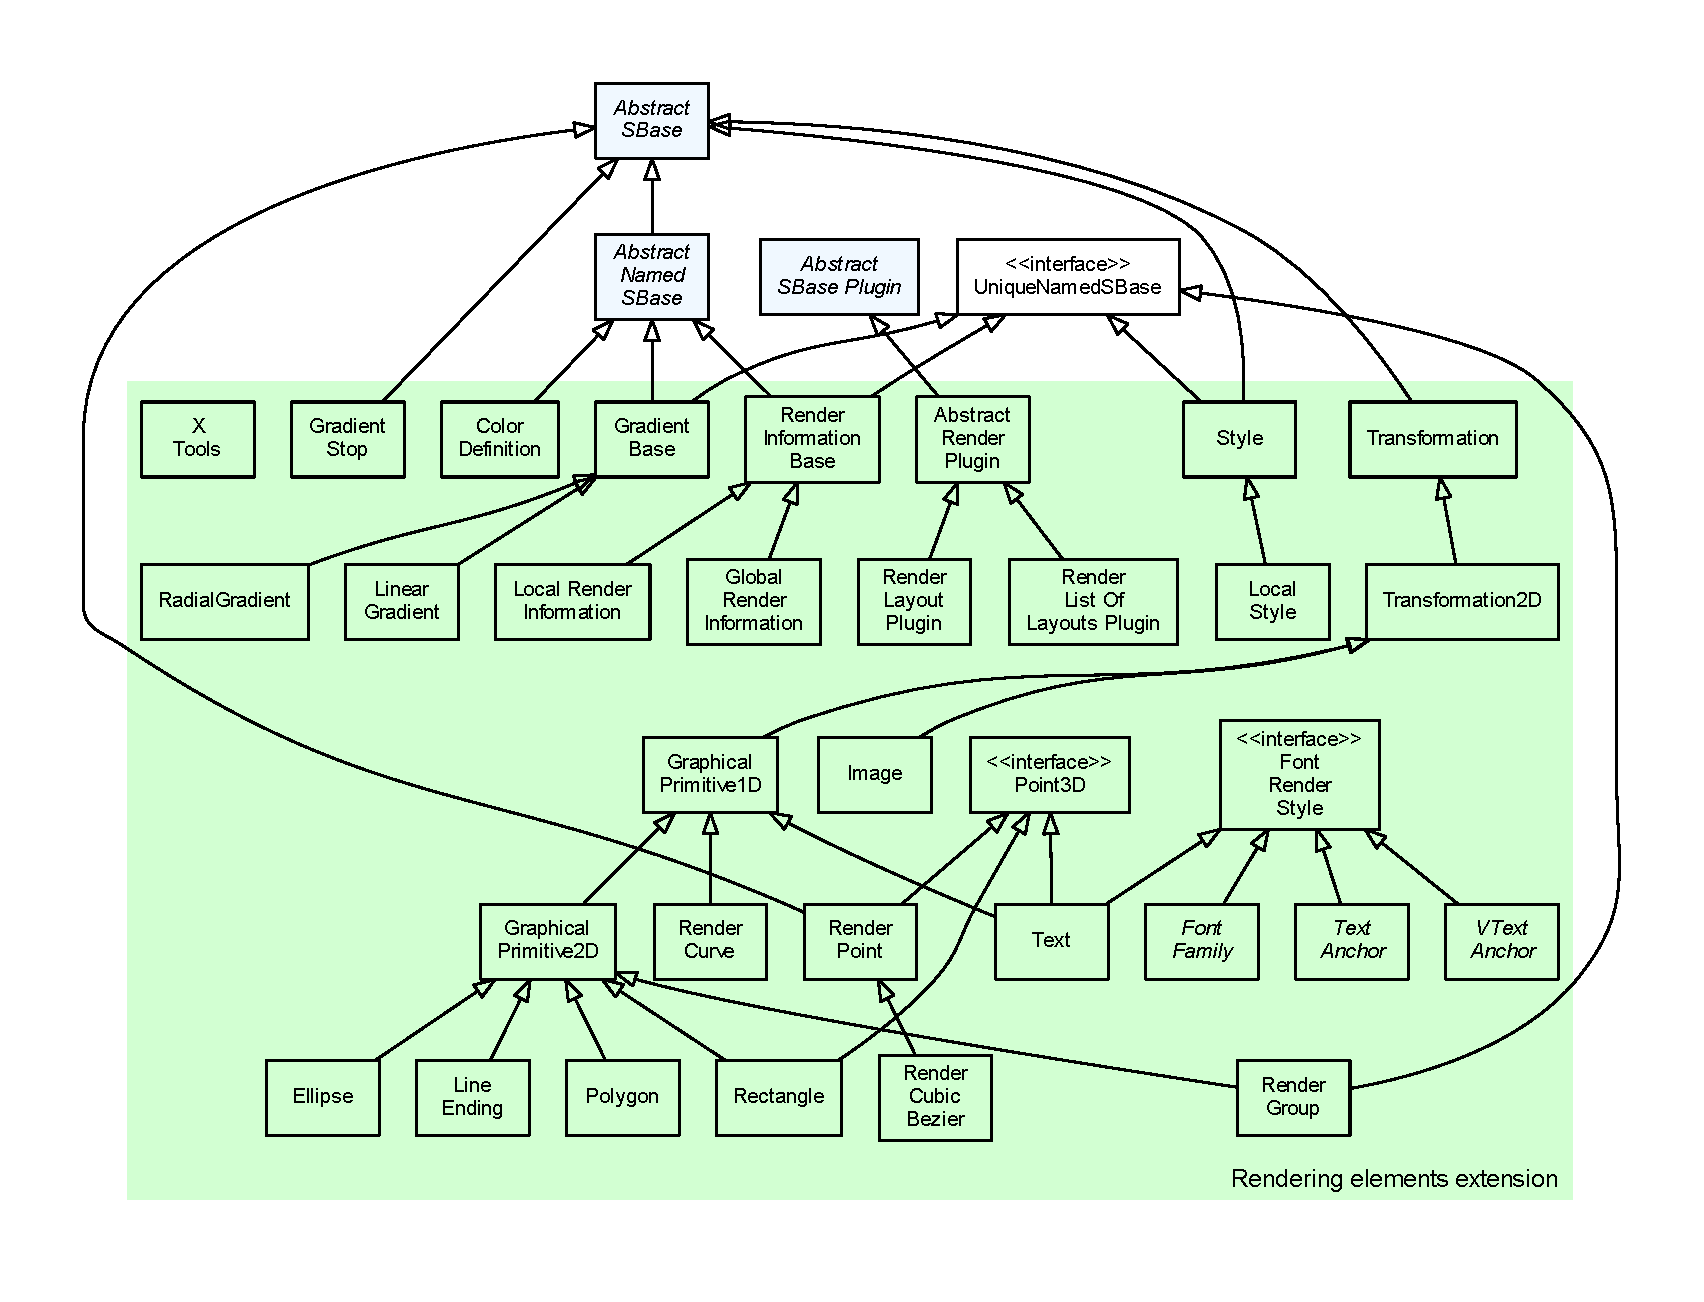
\includegraphics[width=\textwidth]{../../../extensions/render/doc/img/type_hierarchy.pdf}
 \caption[The rendering extension]{}
 \label{fig:render}
\end{figure}
